% ---------------------------------------------------------------------------------------
\chapter{Integración de las componentes de la solución}\label{mldp}
En esta sección se abordará el hardware utilizado para prototipado y diseño de bluetooth bajo consumo (BLE - bluetooth low energy). 

\section{BLEBee}
Para el prototipado se utilizará un módulo bluetooth BLEBee que ofrece una conexión simple a placas Arduino que posean este puerto. 
BLEBee utiliza un módulo de bluetooth RN4020 el cual ofrece bluetooth versión 4.1.\\
Mediante interfaz UART, este modulo puede ser configurado para actuar como módulo central o periférico cuando establezca una conexión.\\
Para conocer mas el funcionamiento de este módulo primero hay que conocer mejor la conexión XBee.

\begin{figure}[H]
\centering
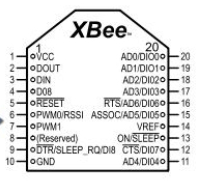
\includegraphics[scale=1]{figuras/bluetooth/xbee.png}
\caption{Forma y Pines de puerto XBee}
\label{xbee}
\end{figure}

Como se puede observar en la figura \ref{xbee} el puerto XBee ofrece una conexión de 20 pines con usos generales que se utilizan por distintos dispositivos, en este caso bluetooth.\\
En el caso de BLEBee la distribución de los pines se puede observar en la figura \ref{blebee}

\begin{figure}[H]
\centering
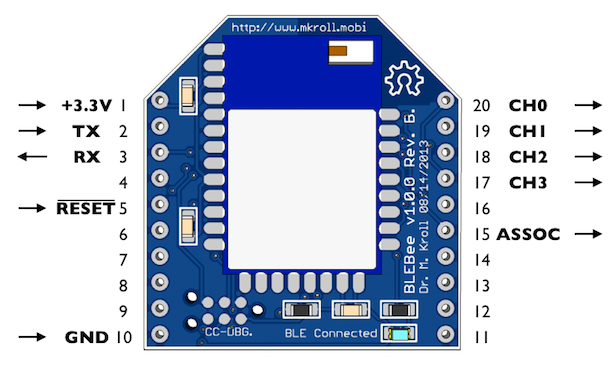
\includegraphics[scale=0.5]{figuras/bluetooth/blebee.png}
\caption{Distribución de pines BLEBee}
\label{blebee}
\end{figure}

Comparando la figura \ref{xbee} con la figura \ref{blebee} se puede observar los pines mas relevantes a la hora de diseñar un módulo bluetooth en el dispositivo, siendo los pines mas importantes, y contrastando con el datasheet, los que se muestran en la tabla \ref{pines}

\begin{table}[H]
\centering
\begin{tabular}{| c | c | c |}
\hline
\multicolumn{1}{|c|}{\textbf{Nº Pin}}&
\multicolumn{1}{c|}{\textbf{Nombre}}&
\multicolumn{1}{|c|}{\textbf{Descripción}}\\ \hline
5  & UART TX & Transmisor UART\\ \hline
6  & UART RX & Receptor UART\\ \hline
7  & WAKE\_ SW & Despertador de modo deep sleep\\ \hline
10 & Led Conexión  & Led indicador de conexión\\ \hline
12 & Led Actividad & Led indicador de actividad\\ \hline
\end{tabular}
\caption{Pines relevantes módulo RN4020}
\label{pines}
\end{table}

\newpage
\section{Comunicación UART}

La comunicación UART (Universal Asynchronous Receiver-Transmitter) es un formato de comunicación serial donde el formato y la velocidad de transmisión son configurables. Un UART puede ser un circuito integrado independiente pero en la actualidad vienen incluidos en los microcontroladores.\\
Para entender mejor como funciona la comunicación serial mediante UART hay que observar la figura \ref{UART}

\begin{figure}[H]
\centering
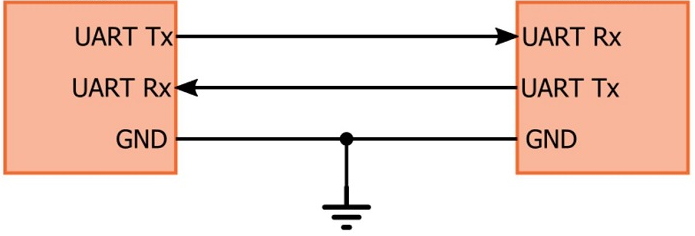
\includegraphics[scale=0.8]{figuras/bluetooth/uart.png}
\caption{Configuración para comunicación UART}
\label{UART}
\end{figure}

La comunicación UART cuenta de 2 pines TX (transmisor) y RX (receptor) el cual se conecta al Receptor y transmisor del microcontrolador respectivamente.

\section{Diseño del módulo bluetooth}
Finalmente contrastando lo visto anteriormente y con referente a la tabla \ref{pines} se puede diseñar el esquemático del integrado.\\
Pin 5 y 6 corresponden a la comunicación UART como se explica en la figura \ref{UART}. Es necesario conectar los pines 10 y 12 con diodos led ya que son pines indicadores, el pin 10 indica el estado de la conexión con un led verde y también se recomienda conectar un led azul al pin 12 para ver el estado de actividad (ej. Si se está enviando información o está dormido).\\
El pin 7 cumple la función de despertar el módulo bluetooth cuando se encuentre dormido emitiendo desde el microcontrolador una señal de $3.3[V]$.\\
\begin{figure}[H]
\centering
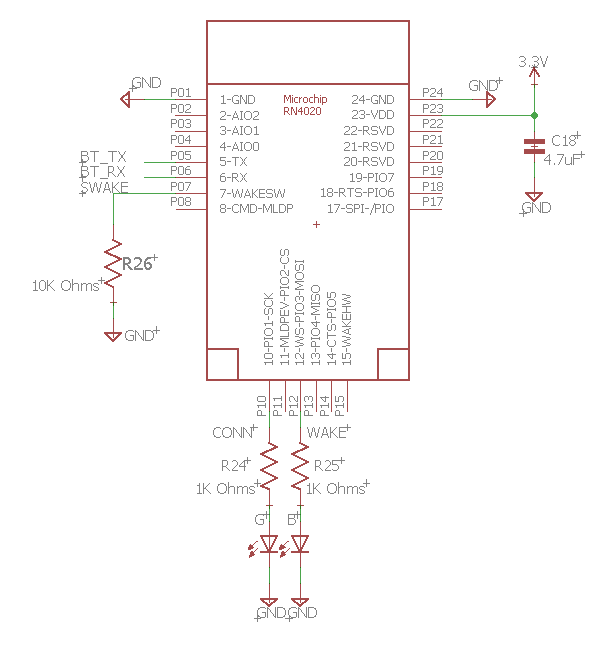
\includegraphics[scale=0.8]{figuras/bluetooth/eagle.png}
\caption{Esquemático bluetooth diseñado en EagleCAD}
\label{eagle}
\end{figure}

Como se puede observar en la figura \ref{eagle} se conecta el módulo bluetooth con los pines descritos. Se utiliza un condensador en la alimentación de módulo para regular el voltaje de la entrada.




